\section{Homework 1}

\subsection{Exercise 2.1}
Showing the definition of convexity for arbitrary $k$. $\theta_1 x_1 + \dots + \theta_k x_k \in C$.
\begin{equation}
  \theta_1 x_1 + \dots + \theta_k x_k = \theta_1 x_1 + (1-\theta_1)(\mu_2 x_2 + \mu_3 x_3 + \dots + \mu_k x_k)
\end{equation}
Where each $\mu_n = \frac{\theta_n}{1-\theta_1}$
\\ \\ 
\begin{equation}
  \sum_i \mu_i = \frac{\sum_i \theta_i}{1-\theta_1} = \frac{1-\theta_1}{1-\theta_1} = 1
\end{equation}
\subsection{Exercise 2.2}
The intersection between any two convex sets is convex. A line segment by definition is convex because it contains itself. Therefore, if there is any line segment $L$ that intersects $C$, for $C$ to be convex, the intersection must also be convex.
\\ \\ 
Similarly, for an affine set, the definition is that the set must contain hte line through any distinct points in the set. Therefore if there is a line that line segment $L$ that intersects an affine set $A$, its intersection is also affine.
\subsection{Exercise 2.5}
Distance between two parallel hyperplanes $\{x \in \mathbb{R}^n | a^T x = b_1 \}, \{x \in \mathbb{R}^n | a^T x = b_2\}$:
\begin{gather}
  a^T(x_1+ at) = b_2 \\
  a^Tx_1 + a^Tat = b_2 \\
  t = \frac{b_2-a^Tx_1}{a^Ta} \\
  t = \frac{b_2 - b_1}{a^Ta} \\
  \frac{|b_1 - b_2|}{||a||_2}
\end{gather}
\subsection{Exercise 2.7}
The image below illustrates the intuition behind this in $\mathbb{R}^2$. The set of all points that are closer to a than b $\{x | ||x-a||_2 \leq ||x-b||_2\}$, is a halfspace of the form 
\begin{equation}
  \{x| c^T x \leq d \}
\end{equation} where $c$ is the normal vector that points from $a$ to $b$, $ c = \frac{a-b}{||a-b||_2}$ and $d = (\frac{a-b}{||a-b||_2})^T \frac{a+b}{2}$
\begin{figure}[htbp]
  \centerline{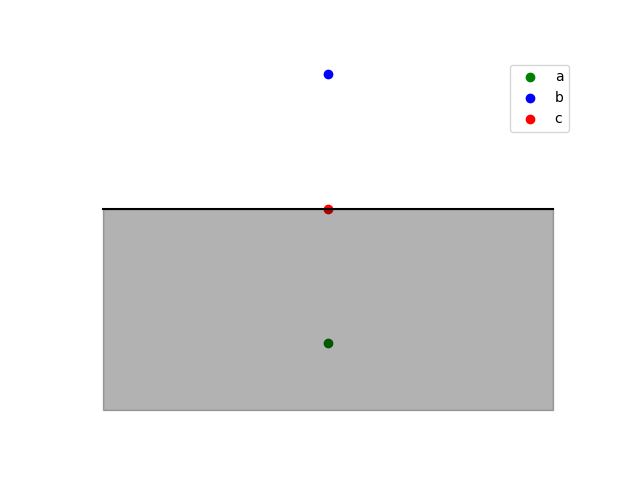
\includegraphics[width=0.75\textwidth]{hw1/images/voronoi_halfspace.png}}
\end{figure}
\subsection{Exercise 2.8}
Finding which of the sets are polyhedra
\subsubsection{a}
S = $\{y_1 a_1 + y_2 a_2 | -1 \leq y_1 \leq 1, -1 \leq y_2 \leq 1 \}, a_1, a_2 \in \mathbb{R}^n$
This set is a 2D parallelogram in any $\mathbb{R}^n$. The image shown is one that is generated with $\mathbb{R}^3$ coordinates $a_1 = (1,2,3) \text{ and } a_2 = (4,5,2)$. It can be defined as the intersection between four halfspaces with their normals pointing from the origin to and centered on $a_1, a_2, -a_1, -a_2$.
\begin{figure}[htbp]
  \centerline{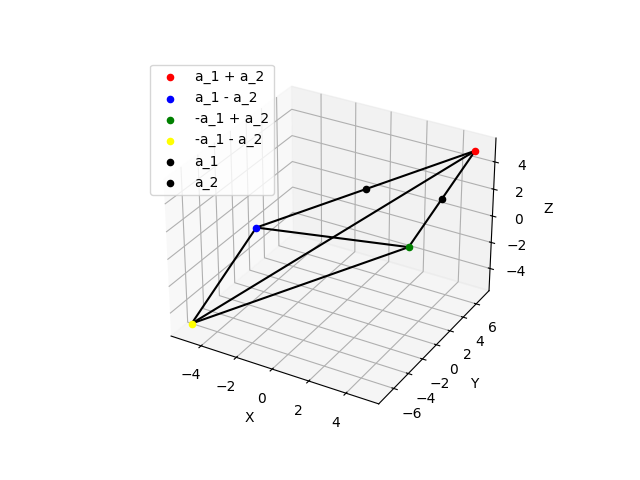
\includegraphics[width=0.5\textwidth]{hw1/images/polyhedra_a.png}}
\end{figure}
\\ \\ 
The normal vectors for the halfspaces are: 
\begin{align}
  A = 
  \begin{bmatrix}
     \frac{a_1}{||a_1||_2} \\
     \frac{a_2}{||a_2||_2} \\ 
     \frac{-a_1}{||a_1||_2} \\
     \frac{-a_2}{||a_2||_2}
  \end{bmatrix}
\end{align}

and the b vector is:
\begin{align}
  b = 
  \begin{bmatrix}
    ||a_1||_2 \\
    ||a_2||_2 \\ 
    ||a_1||_2 \\
    ||a_2||_2
  \end{bmatrix}
\end{align}

Therefore, the set S can be expressed as $S = \{x | Ax \preceq b\}$ 

\subsubsection{b}
This is a polyhedra where:
\begin{gather}
  A = I^n \\
  b = 0
\end{gather}
\begin{align}
  C = 
  \begin{bmatrix}
     \mathbf{1} \\
     a \\
     a^2
  \end{bmatrix}
\end{align}

\begin{align}
  d = 
  \begin{bmatrix}
    1 \\ 
    b_1 \\
    b_2    
  \end{bmatrix}
\end{align}

\subsubsection{c}
Not attempted
\subsubsection{d}
Not attempted

\subsection{Exercise 2.11}
Showing that the hyperbolic set $\{x \in \mathbb{R}^2_{++} | x_1 x_2 \geq 1\}$ is convex. As a generalization, show that $\{x \in \mathbb{R}^2_{+} | \Pi_{i=1}^n x_i \geq 1\}$
\subsection{Exercise 2.12}
Finding which of the following sets are convex:
\subsubsection{a. slab}
A set of the form $\{x \in \mathbb{R}^n | \alpha \leq a^T x \leq \beta\}$,
A slab is the intersection of two halfspaces $\mathbb{C}$ and $\mathbb{D}$ 
where $\mathbb{C} = \{x| a^T x \leq \beta\}$ and $\mathbb{D} = \{x| -a^T x \leq -\alpha\}$  

\subsubsection{b. rectangle}
A set of the form $\{ x \in \mathbb{R}^n | \alpha_i \leq x_i \leq \beta_i, i = 1,\dots, n\}$.
This is also the intersection of halfspaces, but this time it is the intersection of four halfspaces (in $\mathbb{R}^2$). But this is a polyhedra.

\subsubsection{c. wedge}
A set of the form $\{x \in \mathbb{R}^n | a_1^T x \leq b_1, a_2^T x \leq b_2\}$.
Intersection of two halfspaces 

\subsubsection{d. point-set distance}
A set of the form $\{ x |  \| x-x_0 \|_2 \leq \| x-y \|_2 \forall y \in S\}$ where $S \subseteq \mathbb{R}^n$. 
This can be viewed as the intersection of many euclidean balls. The intersection of convex spaces is convex so the here, the set can be turned into $\cap_{y \in S} \{ x |  \| x-x_0 \|_2 \leq \| x-y \|_2\}$
\subsubsection{e. set-set distance}
A set of the form $\{ x | \textbf{dist}(x,S) \leq  \textbf{dist}(x,T) \}$
This set is not convex. Consider two crescent-moon shaped sets that lie next to each other so the tip of one moon is in the center of the other moon. The set that is closer to either of them is not convex because the crescent shape would stay in the set and is not convex.

\subsubsection{f. affine set combo}
A set of the form $\{ x | x + S_2 \subseteq S_1 \}$, where $S_1, S_2 \subseteq \mathbb{R}^n$
Yes, this is essentially the section of $S_2$ that can be translated to the convex $S_1$

\subsubsection{g. fraction distance}
Not attempted


\subsection{Exercise 2.15}
Finding which conditions sets are convex that are conditions on the probability simplex $\{ p | \textbf{1}^T p = 1, p  \succeq 0 \}$:
\subsubsection{a. bounded expectation}
This is a linear bound, so this set is convex.

\subsubsection{b. prob a and b}
Not attempted

